% !TEX root = ../../Rapport/rapport.tex
% !TEX encoding = UTF-8 Unicode


\section{Programmation dynamique}

\subsection{Sur le problème de la partition}
\subsubsection{Condition nécessaire sur la somme des poids des $n$ objets}

Les poids de chacun des objets étant des valeurs entières, pour qu'il existe deux sous-ensembles
distincts ayant le même poids, il faut que la somme des poids des objets soit paire.

\subsubsection{Récurrence}

Introduisons l'expression booléenne $T(i,j) $ : \emph{Etant donnés les $i$ premiers éléments de la
famille, il existe un sous-ensemble de ces $i$ éléments de poids $j$}. 

Dans un premier temps il paraît évident que si $j=0$, le sous-ensemble existe : il s'agit de
l'ensemble vide. \begin{equation}
\forall i \in \mathbb{[}0, n \mathbb{]}, \quad T(i,0) = \mbox{VRAI} 
\end{equation}

De plus, si $j$ est égal au poids de l'un des $i$ premiers éléments, alors l'existence du
sous-ensemble est avérée. Autrement dit, si l'on appelle $K_i$ l'ensemble formé par les poids des
objets $i$, on a : \begin{equation}
	\forall i \in \mathbb{[}0, n \mathbb{]}, \quad T(i,j \in K_i) = \mbox{VRAI}
\end{equation}

Troisièmement, l'ensemble des $i-1$ premiers objets est un sous ensemble de l'ensemble des $i$
premiers objets : $E_{i-1} \subset E_i$. On en déduit donc, que s'il existe un sous ensemble de
$E_{i-1}$ de poids $j$ tel que $T(i-1, j) = \mbox{VRAI}$, alors ce sous-ensemble est aussi un
sous-ensemble de $E_i$ tel que $T(i, j) = \mbox{VRAI}$ et ce par le principe d'inclusion.
\begin{equation}
	\forall i \in \mathbb{[}0, n \mathbb{]}, \quad \mbox{ si } T(i-1, j) = \mbox{VRAI}, \mbox{
	alors } T(i,j) = \mbox{VRAI}
\end{equation}

Enfin, considérons $S_j$ un sous-ensemble de $E_{i-1}$ de pois $j$ vérifiant donc $T(i-1, j) =
\mbox{VRAI}$, alors $S_j \cup a_i$ est un sous-ensemble de $E_i$ de poids $j+p(a_i)$ et donc
vérifiant $T(i,j+p(a_i)) = \mbox{VRAI}$. On en déduit donc :
\begin{equation}
	\forall i \in \mathbb{[}0, n \mathbb{]}, \quad \mbox{ si } T(i-1, j-p(a_i)) = \mbox{VRAI}, \mbox{
	alors } T(i,j) = \mbox{VRAI}
\end{equation}

En réunissant les équations ci dessus dans une seule expression booléenne, on obtient la formule de
la ligne $i$ en fonction de la ligne $i-1$ et $p(a_i)$ :
\begin{equation}
	T(i,j) = j == 0 \vee j == p(a_i) \vee T(i-1, j) \vee T(i-1, j-p(a_i))
\end{equation}

On peut alors donner un algorithme pour résoudre le problème de la partition : l'algorithme
\ref{solvepart}.

\begin{algorithm}[H]
	\caption{Partition}
	\label{algo_dyn_partition}
	\begin{algorithmic}[1]
		\STATE $P \leftarrow \sum_{i \in \mathbb{[}1, n \mathbb{]}} p(a_i)$
		\IF{$P \equiv 1 \pmod{2}$}
			\RETURN Pas de solution
		\ELSE
			\FOR {$j \in \mathbb{[}0,P/2\mathbb{]}$}
				\IF{$j = 0$}
					\STATE $T(0, j) \leftarrow \TRUE$
				\ELSE
					\STATE $T(0, j) \leftarrow \FALSE$
				\ENDIF
			\ENDFOR
			\FOR{$i \in \mathbb{[}1, n \mathbb{]}$}
				\FOR{$j \in \mathbb{[}0, P/2\mathbb{]}$}
					\STATE $T(i, j) \leftarrow [\left (j = 0) \vee (j = p(a_i)) \vee (T(i-1, j)) \vee (T(i-1, j-p(a_i))) \right]$
				\ENDFOR
			\ENDFOR
			\IF{$T(n, P / 2) = \FALSE$}
				\RETURN Pas de solution
			\ELSE
				\RETURN Partition-Solution($n$,$\frac{P}{2}$,$T$)
			\ENDIF
		\ENDIF
	\end{algorithmic}
\end{algorithm}

\begin{algorithm}
	\caption{Partition-Solution}
	\label{recsol}
	\begin{algorithmic}[1]
	\REQUIRE
		\IF{$i = 0$ \OR $j=0$}
			\RETURN $S$
		\ELSE
			\IF{$T(i-1,j) = \FALSE$}
				\RETURN $a_i \cup$ Partition-Solution($i-1$,$j-a_i$,$T$)
			\ELSE
				\RETURN Partition-Solution($i-1$, $j$, $T$)
			\ENDIF
		\ENDIF
	\end{algorithmic}
\end{algorithm}



Le sous ensemble solution $S_{sol}$ se construit à l'aide du principe suivant : pour une ligne $i>0$ et
un poids $j>0$ donnés, on a $a_i \in S_{sol}$ si $T(i-1, j) = \mbox{FAUX} \wedge T(i,j) =
\mbox{VRAI}$. Ceci n'est vrai que dans un sens et permet d'introduire l'implication suivante :
\begin{equation}
	\label{ineq}
	T(i-1, j) \oplus T(i, j) = \mbox{VRAI} \Rightarrow a_i \in S_{sol} 
\end{equation}

Ceci mérite quelques explications. Séparons les différents cas possibles et présentons les dans un
tableau : \\
\begin{center}
\begin{tabular}{|c|c|c|} \hline
	\backslashbox{$T(i-1, j)$}{$T(i,j)$} & VRAI & FAUX \\	\hline
	VRAI & Cas 1 & Cas 2 \\ \hline
	FAUX & Cas 3 & Cas 4 \\ \hline
\end{tabular}
\end{center}

Analysons les différents cas : \begin{enumerate}
	\item Dans ce cas, l'ensemble des $i-1$ premiers objets possède un sous-ensemble vérifiant les
		contraintes imposées. On peut donc en déduire qu'il existe un sous-ensemble ne contenant pas
		$a_i$ et vérifiant ces mêmes contraintes\footnote{Attention, celà ne veut pas dire qu'il
		n'existe pas de sous-ensembles vérifiant les contraintes et contenant $a_i$}. C'est cet ensemble
		qui nous intéresse
	\item Ce cas est un cas interdit par la formule de calcul de la ligne $i$. En effet, si $T(i-1, j)
		=$ VRAI, alors $T(i,j) =$ VRAI par construction.
	\item C'est ce cas qui est intéressant, puisqu'il nous indique que l'ajout de l'objet $a_i$ permet
		de trouver une solution au problème du sous-ensemble pour les valeurs données. On a donc $a_i$
		appartenant bel et bien à la solution.
	\item Ce cas indique juste que que la solution n'existe pas.
\end{enumerate}
~\\
De ces principes, on peut déduire l'algorithme \ref{recsol} de reconstruction de la solution.

\subsubsection{Complexité}
$O(n.P)$
%TODO

\subsubsection{Jeux d'essais}


\subsection{Le problème du sac à dos}

\begin{algorithm}[H]
	\caption{Sac à Dos}
	\label{algo_dyn_bag}
	\begin{algorithmic}[1]
		\FOR {$j \in \mathbb{\{}1, \ldots, volumeMax \mathbb{\}}$}
				\STATE $T[0, j] \leftarrow 0$
		\ENDFOR
		\FOR{$i \in \mathbb{\{}1, \ldots, n \mathbb{\}}$}
			\FOR{$j \in \mathbb{\{}1, \ldots, volumeMax \mathbb{\}}$}
				\IF{$j \neq 1$}
					\STATE $T[i, j] \leftarrow T[i, j-1]$
				\ENDIF
				\FOR{$k \in \mathbb{\{}0, \ldots, volumeMax/volume[i] \mathbb{\}}$}
					\STATE $T[i,j] \leftarrow \max(T[i,j], T[i-1,j-k \times volume[i]] + k \times utilite[i])$
				\ENDFOR
			\ENDFOR
		\ENDFOR
	
	\RETURN $T[n,volumeMax]$
	\end{algorithmic}
\end{algorithm}



\subsubsection{Justification des formules}

\subsubsection{Exemple}

Considérons le problème suivant :
Le sac à dos a une capacité de 6 et les propriétés des objets sont définies dans le tableau suivant
:
\begin{center}
\begin{tabular}{|c|c|c|c|c|} \hline
	utilité & 1 & 3 & 4 & 5 \\ \hline
	volume & 1 & 4 & 2 & 2 \\ \hline
\end{tabular}
\end{center}

L'algorithme va donc créer la matrice suivante :
\begin{center}
$$\begin{array}{|c|c|c|c|c|c|c|} \hline
  _{objet}^{volume} & 1 & 2 & 3 & 4 & 5 & 6 \\ \hline
	0		  & 0 & 0 & 0 & 0 & 0 & 0 \\ \hline
	1			& 1 \times i_1 = 1 & 2 \times i_1 = 2 & 3 \times i_1 = 3 & 4 \times i_1 = 4 & 5 \times i_1 = 5 & 6 \times i_1 = 6 \\ \hline
	2			& 1 \times i_1 = 1 & 2 \times i_1 = 2 & 3 \times i_1 = 3 & 4 \times i_1 = 4 & 5 \times i_1 = 5 & 6 \times i_1 = 6 \\ \hline
	3			& 1 \times i_1 = 1 & 1 \times i_3 = 4 & 1 \times i_1 + 1 \times i_3 = 5 & 2 \times i_3 = 8 & 1 \times i_1 + 2 \times i_3 = 9 & 3 \times i_3 = 12 \\ \hline
	4			& 1 \times i_1 = 1 & 1 \times i_3 = 4 & 1 \times i_1 + 1 \times i_4 = 6 & 2 \times i_4 = 10
	& 1 \times i_1 + 2 \times i_4 = 11  & 3 \times i_4 = 15 \\ \hline
\end{array}$$
\end{center}

Il ne nous reste plus qu'à lire la solution optimale dans la case [4,6].


\subsubsection{Complexité}
Notre algorithme génère une matrice de taille $n \times V$, et pour chaque case dans le pire des cas (si $v_i = 1$), il faudra $V$ 
itérations. Ainsi nous obtenons la complexité en temps suivante : $\bigcirc(n\times V^2)$.
De plus, si la matrice est stockée entièrement, la complexité en espace est donc en $\bigcirc(n\times V)$.

\subsection{Le problème du voyageur de commerce}

\begin{algorithm}[H]
	\caption{Voyageur de Commerce}
	\begin{algorithmic}[1]
		\FOR{$i \in \{1,...,n\}$}
			\STATE $C(\{0\},i) \leftarrow \omega(0,i)$
		\ENDFOR
		\FOR{$i \in \{2,...,n\}$}
			\FOR{$S \subseteq \{1,...,n\} : |S| = i$}
				\FOR{$j \in V \setminus S$}
					\STATE $C(S,j) \leftarrow \min\limits_{k \in S \setminus \{0\}}(C(S\setminus\{k\},k) + \omega(k,j))$
				\ENDFOR
			\ENDFOR
		\ENDFOR
		\RETURN $\min\limits_{i\in V\setminus\{0\}}(C(V\setminus\{i\},i) + \omega(i,0))
	\end{algorithmic}
\end{algorithm}



\subsubsection{Exemple}
% !TEX root = ../../rapport/rapport.tex

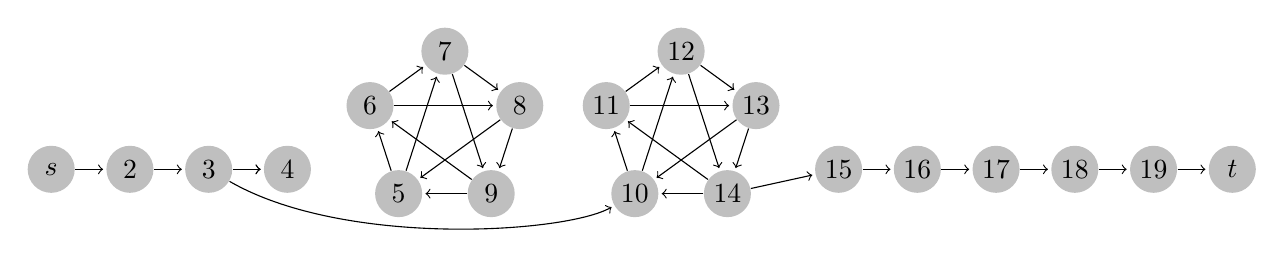
\begin{tikzpicture}[shorten >=1pt,->]
  \tikzstyle{vertex}=[circle,fill=black!25,minimum size=17pt,inner sep=0pt]

  \foreach \name/\x in {s/1, 2/2, 3/3, 4/4, 15/11, 
                        16/12, 17/13, 18/14, 19/15, t/16}
    \node[vertex] (G-\name) at (\x,0) {$\name$};

  \foreach \name/\angle/\text in {P-1/234/5, P-2/162/6, 
                                  P-3/90/7, P-4/18/8, P-5/-54/9}
    \node[vertex,xshift=6cm,yshift=.5cm] (\name) at (\angle:1cm) {$\text$};

  \foreach \name/\angle/\text in {Q-1/234/10, Q-2/162/11, 
                                  Q-3/90/12, Q-4/18/13, Q-5/-54/14}
    \node[vertex,xshift=9cm,yshift=.5cm] (\name) at (\angle:1cm) {$\text$};

  \foreach \from/\to in {s/2,2/3,3/4,3/4,15/16,16/17,17/18,18/19,19/t}
    \draw (G-\from) -- (G-\to);

  \foreach \from/\to in {1/2,2/3,3/4,4/5,5/1,1/3,2/4,3/5,4/1,5/2}
    { \draw (P-\from) -- (P-\to); \draw (Q-\from) -- (Q-\to); }

  \draw (G-3) .. controls +(-30:2cm) and +(-150:1cm) .. (Q-1);
  \draw (Q-5) -- (G-15);
\end{tikzpicture}



{\bf i = 1}\\
\begin{center}
$$\begin{array}{|c|c|} \hline
	_i^S & \{0\} \\ \hline
	1 & \{0,1\} = 1\\ \hline
	2 & \{0,2\} = 2\\ \hline
	3 & \{0,3\} = 1\\ \hline
	4 & \{0,4\} = 0\\ \hline
\end{array}$$
\end{center}


{\bf i = 2}\\
\begin{center}
$$\begin{array}{|c|c|c|c|c|} \hline
	_i^S & \{0,1\} & \{0,2\} & \{0,3\} & \{0,4\} \\ \hline
	1 & $\ding{55}$ & \{0,2,1\} = 5 & \{0,3,1\} = 6& \{0,4,1\} = 0\\ \hline
	2 & \{0,1,2\} = 4 & $\ding{55}$ & \{0,3,2\} = 3& \{0,4,2\} = 1\\ \hline
	3 & \{0,1,3\} = 6 & \{0,2,3\} = 4 & $\ding{55}$ & \{0,4,3\} = 4\\ \hline
	4 & \{0,1,4\} = 1 & \{0,2,4\} = 3 & \{0,3,4\} = 5& $\ding{55}$\\ \hline
\end{array}$$
\end{center}

{\bf i = 3}\\
\begin{center}
$$\begin{array}{|c|c|c|c|c|c|c|} \hline
	_i^S & \{0,1,2\} & \{0,1,3\} & \{0,1,4\} & \{0,2,3\}
& \{0,2,4\}& \{0,3,4\} 
\\ \hline
	1 & $\ding{55}$ & $\ding{55}$ & $\ding{55}$ & \{0,3,2,1\} = 6
& \{0,2,4,1\} = 3 & \{0,3,4,1\} = 5 \\ \hline
	2 & $\ding{55}$ & \{0,1,3,2\} = 8 & \{0,1,4,2\} = 2 & $\ding{55}$ 
& $\ding{55}$ & \{0,3,4,2\} = 6 \\ \hline
	3 & \{0,1,2,3\} = 6 & $\ding{55}$ & \{0,1,4,3\} = 5 & $\ding{55}$
& \{0,4,2,3\} = 3 & $\ding{55}$ \\ \hline
	4 & \{0,1,2,4\} = 5 & \{0,3,1,4\} = 6 & $\ding{55}$ & \{0,3,2,4\} = 4 
& $\ding{55}$ & $\ding{55}$ \\ \hline
\end{array}$$
\end{center}

{\bf i = 4}\\
\begin{center}
$$\begin{array}{|c|c|c|c|c|} \hline
	_i^S & \{0,1,2,3\} & \{0,1,2,4\} & \{0,1,3,4\} & \{0,2,3,4\} \\ \hline
	1 & $\ding{55}$ & $\ding{55}$ & $\ding{55}$ & \{0,3,2,4,1\} = 4 \\ \hline
	2 & $\ding{55}$ & $\ding{55}$ & \{0,1,4,3,2\} = 7 & $\ding{55}$ \\ \hline
	3 & $\ding{55}$ & \{0,1,4,2,3\} = 4 & $\ding{55}$ & \ding{55} \\ \hline
	4 & \{0,3,2,1,4\} = 5 & $\ding{55}$ & $\ding{55}$ & \ding{55} \\ \hline
\end{array}$$
\end{center}

Solution optimale : $\{0,3,2,1,4,0\} = 5$.

\subsubsection{Complexité}
La matrice générée ici est de taille $n,2^n$, et il faut $\bigcirc(n)$ opérations pour remplir une case.
Les complexités sont donc :
\begin{itemize}
	\item temps : $\bigcirc(n^2\times 2^n)$
	\item espace : $\bigcirc(n\times 2^n)$
\end{itemize}

